\documentclass[10pt,oneside,a4paper,final,english]{memoir}

\usepackage{palatino}
\usepackage{microtype}
\usepackage{lscape}
\usepackage{multicol}
%\usepackage{epic,eepic}
\usepackage{latexsym}
\usepackage{verbatim}
\usepackage{listings}
\usepackage{ulem}
\usepackage{hyperref}

\let\footruleskip\undefined
\usepackage{fancyhdr}
\usepackage[final]{fixme}

\let\fref\undefined
\usepackage[plain]{fancyref}

%% FOR LOOP
\usepackage{ifthen,calc}
\newcounter{myforloopcounter}
\newcommand{\forloop}[5][1]% 
{\setcounter{#2}{#3}% 
\ifthenelse{#4}% 
{#5%
  \addtocounter{#2}{#1}% 
  \forloop[#1]{#2}{\value{#2}}{#4}{#5}% 
}%
% Else 
{}%
}% 


%% USAGE
%\forloop[step]{counter}{initial_value}{conditional}{code_block} 
\usepackage[english]{babel}
\usepackage[utf8]{inputenc}

%\selectlanguage{danish}

\lstset{language=Python,basicstyle=\small,
  columns=fullflexible}


\usepackage[pdftex]{graphicx}

\DeclareGraphicsExtensions{.jpg .png .pdf}


\usepackage{amsmath}
\usepackage{latexsym}
\usepackage{amssymb}


\usepackage[osf,sc]{mathpazo}
\usepackage{microtype}
%\usepackage{fourier}
\linespread{1.05}

%\usepackage[charter]{mathdesign}
%\usepackage{lmodern}

%\usepackage{algorithmic}
%\usepackage{algorithm}

\usepackage{amsthm}


\theoremstyle{plain}  \newtheorem{definition}{Definition}
\theoremstyle{remark} \newtheorem{lemma}{Lemma}
\theoremstyle{plain}  \newtheorem{theorem}{Theorem}
\theoremstyle{remark}  \newtheorem{example}{Example}


\newcommand{\p}{\ensuremath{^\prime}}
\DeclareGraphicsExtensions{.jpg, .eps, .png}
%%% Local Variables:
%%% mode: plain-tex
%%% TeX-master: "../master"
%%% End:

\usepackage{algorithmic}
\usepackage{algorithm}
\usepackage[sectionbib,square]{natbib}
%\bibpunct{(}{)}{,}{a}{}{}
\setcitestyle{alpha}
%\setcitestyle{numbers,aysep={},yysep={;}}

\usepackage{datetime}

\chapterstyle{thatcher}

\setcounter{secnumdepth}{0}
\setcounter{tocdepth}{0}




%\pagestyle{fancy}
\begin{document}
  \fontencoding{T1}
%  \fontseries{m}
%  \fontshape{n}
%  \fontsize{12}{15}
%  \selectfont


%%%%%%%%%%%%%%%%%%%%%%%%%%%%%%%%%%%%%%%%%%%%%%%%%%%%%%%%
%                    Forside
%%%%%%%%%%%%%%%%%%%%%%%%%%%%%%%%%%%%%%%%%%%%%%%%%%%%%%%%
\makeatletter % open mode for reading @ signed variables
\def\maketitle{%
 \null
 \thispagestyle{empty}%
 \vfill
 \begin{center}\leavevmode
   \normalfont
   \LARGE{\raggedleft \@title\par}%
   \hrulefill\par
   \large{\raggedleft \subtitle\par}%
   \vskip 2cm
   {\today\par}%
 \end{center}%
 \vfill
 \begin{flushleft}
   {\large \@author } \\
   {\footnotesize \suplementInfo }
 \end{flushleft}
 \clearpage % Terminates the page here. Everything else vil be placed
            % on next page.
}
\makeatother % closing mode for reading @ signed variables
%%%%%%%%%%%%%%%%%%%%%%%%%%%%%%%%%%%%%%%%%%%%%%%%%%%%%%%%
%               Data til forside
%%%%%%%%%%%%%%%%%%%%%%%%%%%%%%%%%%%%%%%%%%%%%%%%%%%%%%%%
\title{Final Hand In $\cdot$ Week VIII}

\def\subtitle{CCO $\cdot$ Constraint Continuous Optimization}

\author{Johan Sejr Brinch Nielsen} \def\suplementInfo{

\kern 5pt \hrule width 11pc \kern 5pt

\begin{tabular}{ll}
Email: & zerrez@diku.dk  \\
Cpr.:  & 260886-2547
\end{tabular}

% putter 5pt spacing oven over og neden under stregen
\kern 5pt \hrule width 11pc \kern 5pt

Dept. of Computer Science,  \\
University of Copenhagen

}


\maketitle
\newpage

\section{Introduction}
The goal of this assignment was to implement the DogLeg method and
compare this to the two methods implemented so far.

\section{Trust Region Methods}
As we have seen in earlier studies of optimization methods an easy to
compute decent direction can be found in the inverse direction of the
gradient, that being $-g$. However, using this direction does not come
without complications. First, the direction is only guaranteed to
decent within some $\epsilon$ of the original point. Secondly, even if
one finds an $\epsilon$ that yields the greatest decent in the
objective function and follows this to what is known as the Cauchy
point, the method can still be slow; zigzagging its way to a local
minimum.

An alternative search direction is Newton's direction. As many other
line search methods it uses a search direction described by:
\[ p_k = -B^{-1} \nabla f(x_k) \]

Both of these methods are line search methods. They compute a decent
direction and then decides on an appropriate step size. The method
investigated in this assignment is known as a trust region method. Put
shortly, it decides on a step size and then compute the a decent
direction within the step size (the ``region'').

The idea is to use a model function $m$ that approximates the
objective function $f$. Knowing the step size $\lambda$, the goal is
to find the best search direction in the model function (which is easy
to minimize) and then follow this direction in $f$. Of cause one needs
to verify that the model is in fact precise enough to yield a decent
in $f$. If not, the $\lambda$ is lowered. $\lambda$ is a measure for
the precision of the model function. The region containing points with
a distance lower than $\lambda$ away from $x_k$ is called the
``trust'' region.


\section{Dog-Leg Method}
The Dog-Leg method is based on a combination of the Cauchy point and a
Quasi-Newton method. It uses a second degree Taylor expansion as its
model. It will choose its search direction based on the following
three cases:
\begin{enumerate}
\item When the point suggested by Newton's method is within the trust
  region, this point is selected.
\item If this is not the case and the trust region requests a smaller
  step than that of the Cauchy point, the direction towards this point
  is followed as far as the region permits.
\item In the third case, when the region boundary is between the
  Cauchy point and the Newton point, the intersection between the
  limiting boundary and the line between these two points are chosen.
\end{enumerate}

As can be seen, the possible directions is given by two joined lines
(from $p_k$ to the Cauchy point and further to Newton's point). This
gives a bending line (a ``dog leg''). Note that since the model
function is quadratic, the Newton method will minimize it in a single
iteration. So there is never a need to go further than the point found
by Newton's method.

Specifically, $p_k$ may take one of the following forms:
\begin{enumerate}
\item \[ p_{k+1} = p^B \]
\item \[ p_{k+1} = \frac{\Delta}{\mid p^U\mid}  p^U \]
\item \[ p_{k+1} = p^U + \frac{\Delta - \mid p^U\mid}{
    \mid p^B\mid + 2p^{U\prime} p^B} p^B \]
\end{enumerate}

Where $\Delta$ is the size of the trust region, $p^B$ is the point
suggested by Newton's method and $p^U$ is the Cauchy point. The two
latter points are defined as:
\[ p^B = -B^{-1} \cdot g \]
\[ p^C = \frac{g' g}{g'Bg} \cdot g \]

Where $g$ is the gradient in the point $x_k$, $B$ is an approximation
of the Hessian and $B^{-1}$ is an approximation of its inverse; both
$B$ and $B^{-1}$ are positive definite matrices.

There is one detail in the algorithm yet to be discussed. That is what
size to choose for $\lambda$ and how to adjust this
dynamically. Generally, one should lower $\lambda$ when no decent
direction is found and only raise $\lambda$ when the step taken is as
long as $\lambda$. In the implementation this is achieved by comparing
the actual improvement in the objective function with that of the
model (the expected improvement).


\section{Verification}
The implementation provided contains an odd bug. Apparently, the
following expression becomes negative:
\[ \frac{g'g}{g'B g} \]

Because of this, the Cauchy point is computed to be in the opposite
direction of $-g$, hence in a non-decending direction.

I have failed to figure out why this bug occurs. All I can say is,
that it is periodically and that it affects the results presented in
this section. The fix is quick and dirty. I have used the ``abs''
function to ensure non-negativity of ``B''.

In the following I present and discuss my experimental results.

\begin{center}
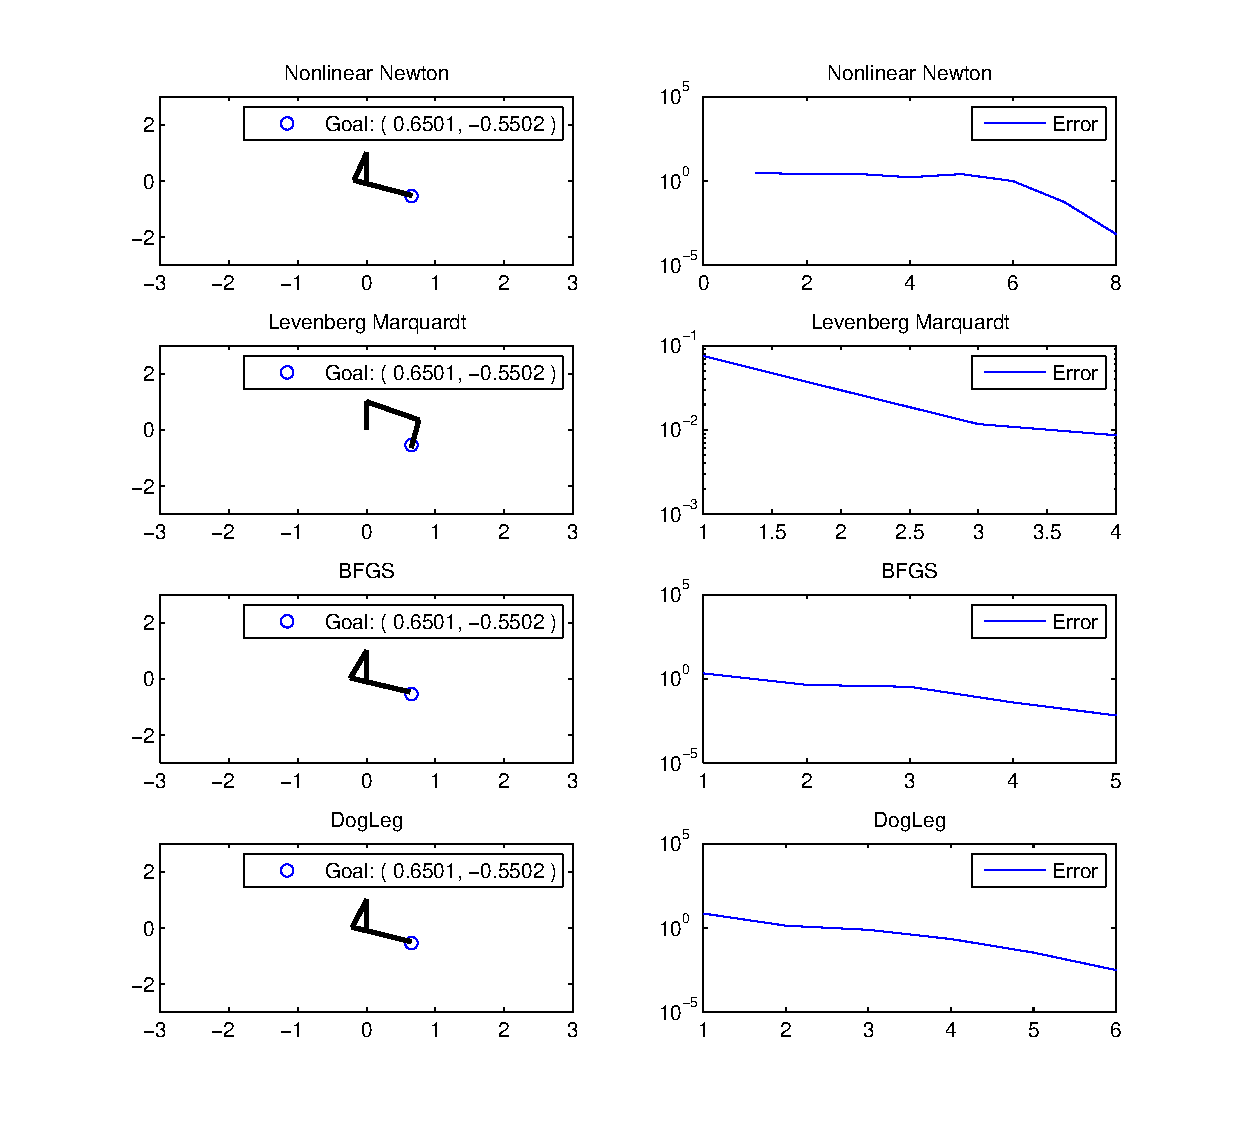
\includegraphics[width=\textwidth]{images/graph0.pdf}
\end{center}

This first problem is solved effeciently by all methods. Apparently
not much of a challenge, but a nice test to see that something does in
fact work; despite the bug. The number of iterations are too few to
say anything useful, except that the Dog-Leg method does not perform
significantly worse than the others.


\begin{center}
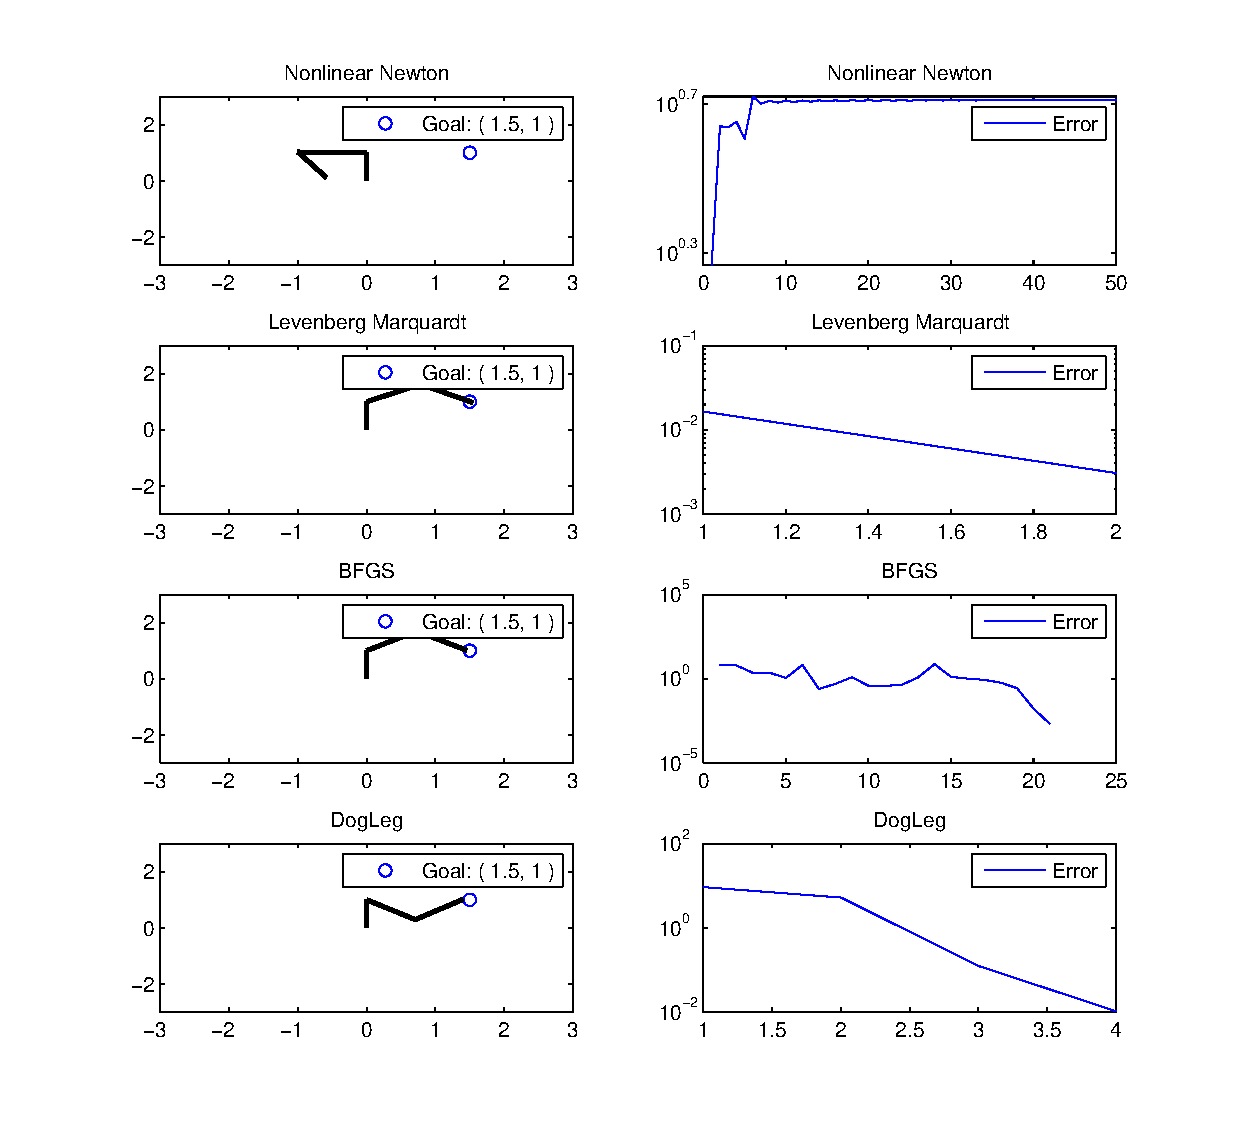
\includegraphics[width=\textwidth]{images/graph1.pdf}
\end{center}

Here Newton's method alone fails to find the point, while Dog-Leg that
is a combination of a Quasi-Newton method and the steepest descent
finds a solution in just 4 iterations. Levenberg Marquardt is even
faster with just two iterations.


\begin{center}
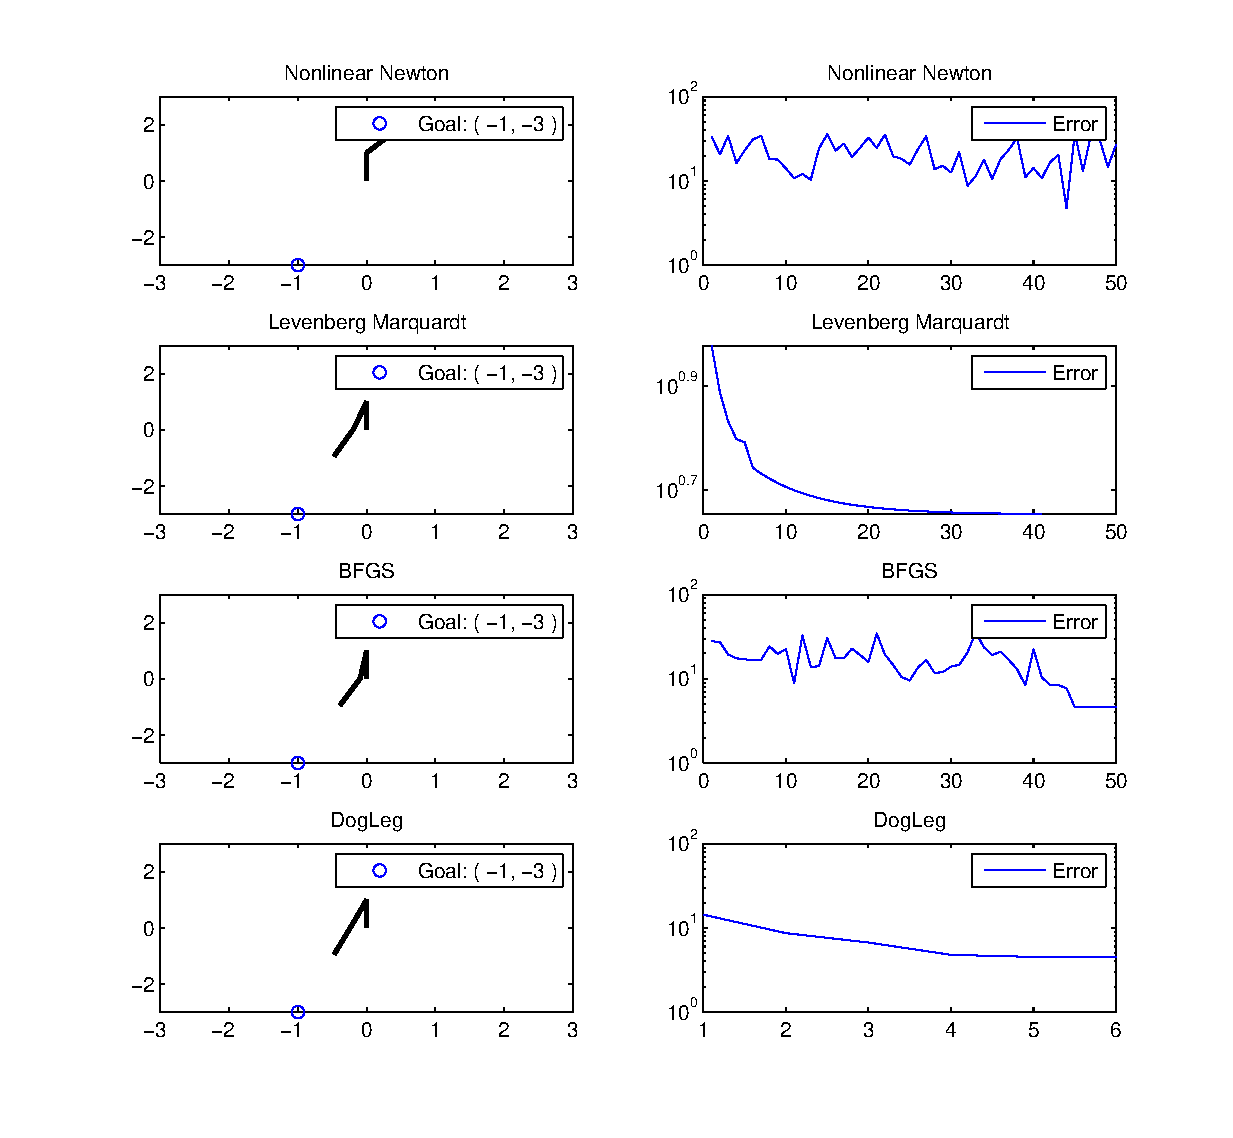
\includegraphics[width=\textwidth]{images/graph3.pdf}
\end{center}

Here is an interesting plot. While Newton's method is simple off
course, Levenberg-Marquardt and BFGS spends all 50 iterations finding
a solution. Dog-Leg uses 6. This suggests that Dog-Leg is more stabile
than the other methods. It uses very few iterations to reach the goal
even as the problems vary. It seems to be a very good all-round
method.

\begin{center}
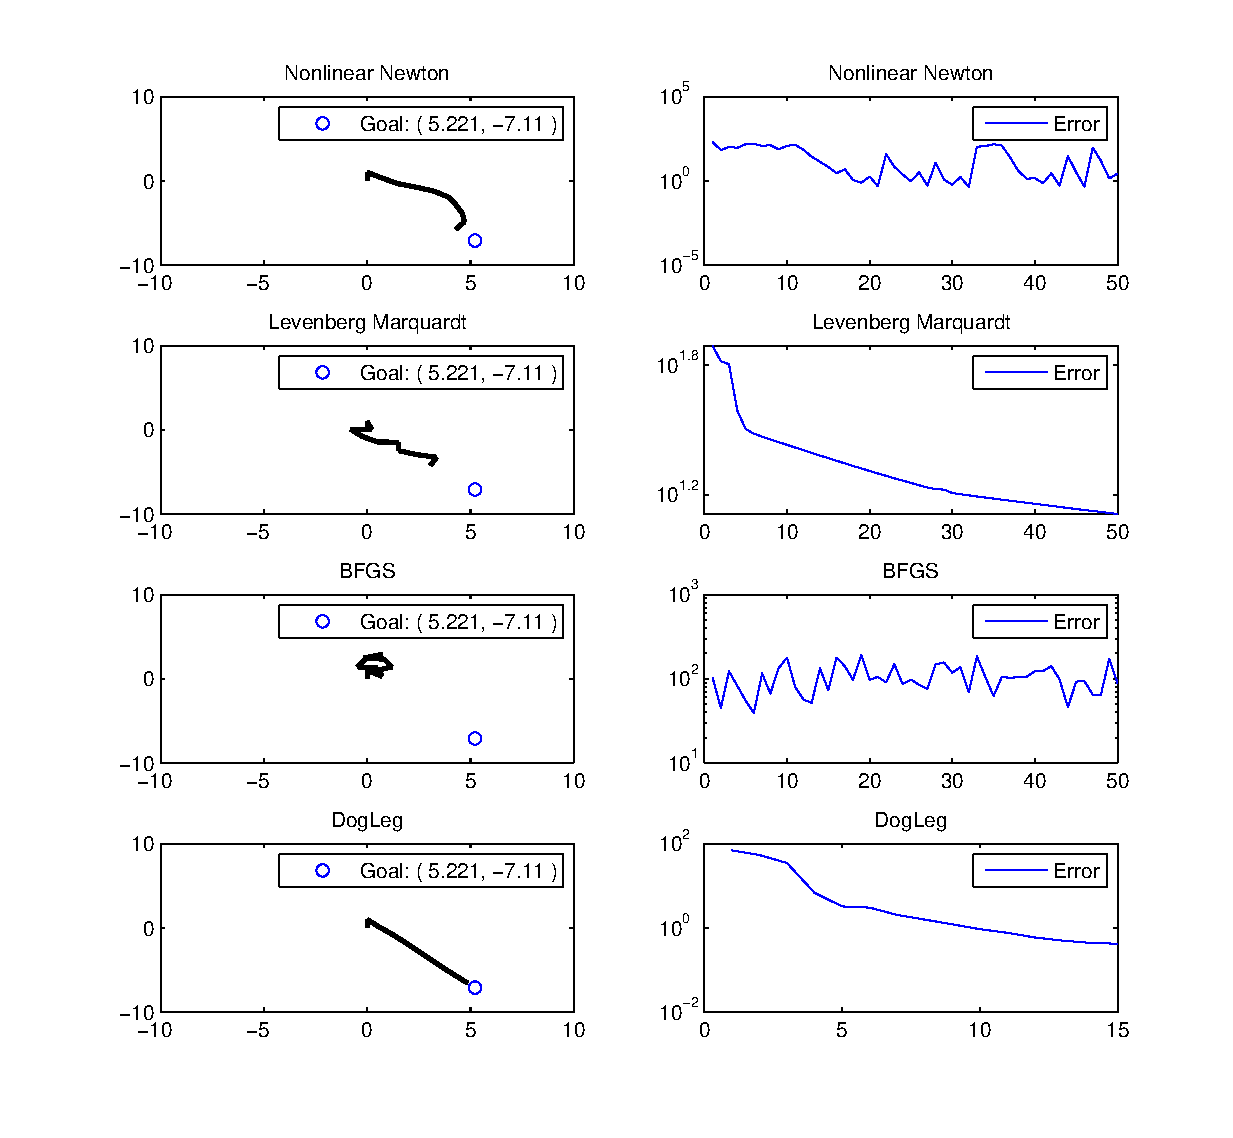
\includegraphics[width=\textwidth]{images/graph5.pdf}
\end{center}
As a final experiment I increase the number of angles to 10. Here it
is clear that the newly implemented Dog-Leg wins. In just 15
iterations it has a path to the goal. The other three methods use all
50 iterations and even though Newton's method is close, it's result is
clearly worse than that of Dog-Leg.



\section{Conclusion}
I have described and implemented the Dog-Leg method, though some
irritating bug has crawled into the code. This has stolen a
significant amount of my time (tracing and fixing) resulting in less
experimentation with the method as I had wanted.

Also, the applied fix affects the chosen direction in a way that may
render the results presented in the verification section invalid.

However, despite all this, the implemented method is extremely fast in
the tested problems and uses just a few iterations, even when the
other methods are in trouble. So, not just does it avoid calculation
of the hessian and inverses - hence, has fast iterations - it will
also find the solution in less iterations. It's simply too good to be
true. I know where I will put my money :-)

The method may work differently, when correctly implemented.



\section{Source Code}
This section contains the MatLab code for the BFGS implementation. I
also updated the source code for the other two methods slightly,
however I considered the changes too small to include here.

\subsection{Run}
\verbatiminput{../code/run.m}

\subsection{Plotit}
\verbatiminput{../code/plotit.m}

\subsection{DogLeg Method}
\verbatiminput{../code/dogleg.m}


\end{document}

%%% Local Variables:
%%% mode: latex
%%% TeX-master: t
%%% End:
